\documentclass[10pt]{article}

\usepackage{spheric}
%%%TITLE
\title{Multiphase Godunov-typed Smoothed Particle Hydrodynamics Method with Approximate Riemann Solvers}
\date{}

\author[1]{Z.W.Cai$^\dagger$}
\author[2]{Z. Zong}
\author[2]{L. Zhou}
\author[3]{Z. Chen}
\author[1]{C.Tiao}

\affil[1]{Department of Offshore Structures, China Ship Scientific Research Center, China}
\affil[2]{School of Naval Architecture, Dalian University of Technology, China}
\affil[1]{Department of Mechanical Engineering, National University of Singapore, Singapore}

\affil[$\relax$]{\email{\dagger}{caizhiwen0904@163.com}}


%%DOCUMENT
\begin{document}

\maketitle

%\SelectedTopics{}

%%PLEASE PUT YOUR ABSTRACT HERE
\begin{abstract}
In this paper, we propose a Multiphase Godunov-typed Smoothed Particle Hydrodynamics
(MGSPH) method for simulating multi-fluid Riemann problems. In this method, different EOSs are
applied on different materials; and interfacial approximate Riemann solvers are introduced on the
interfacial particle pairs to deal with the transition between different EOSs. Various combinations of
five kinds of single-phase approximate Riemann solvers (LLXF, ROE, HLLE, HLLC, DUCO) and
three types of interface approximation Riemann solvers (ROE, LRS, RRS) are comparatively studied
in three numerical tests. It turns out that LLXF and HLLE give worse results than other approximate
Riemann solvers; and pressure instabilities are observed when applying RRS on interfacial particle
pairs. In general, the combinations of DUCO+ROE and DUCO+LRS may be the suitable choices for
MGSPH in simulating multiphase Riemann problems.

\begin{figure}[!htb]
\centering
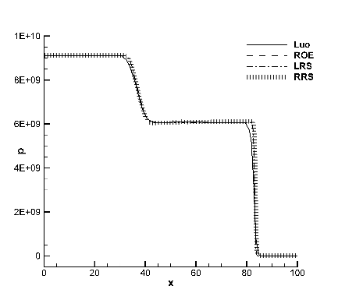
\includegraphics[width=0.46\textwidth]{24-11.png}~~
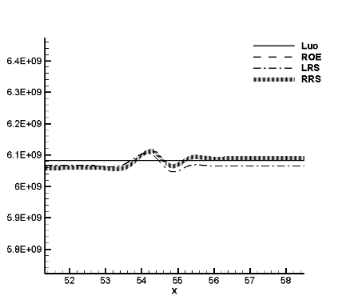
\includegraphics[width=0.46\textwidth]{24-12.png}
\caption{Gas-water shock tube problem. The solutions of $t=0.000156$. Left: pressure; right: broken features}\label{fig:}
\end{figure}

\end{abstract}


%%THE END OF ABSTRACT

%\addbib

\end{document}
